%
% fig-kruemmung.tex
%
% (c) 2025 Prof Dr Andreas Müller
%
\begin{figure}
\centering
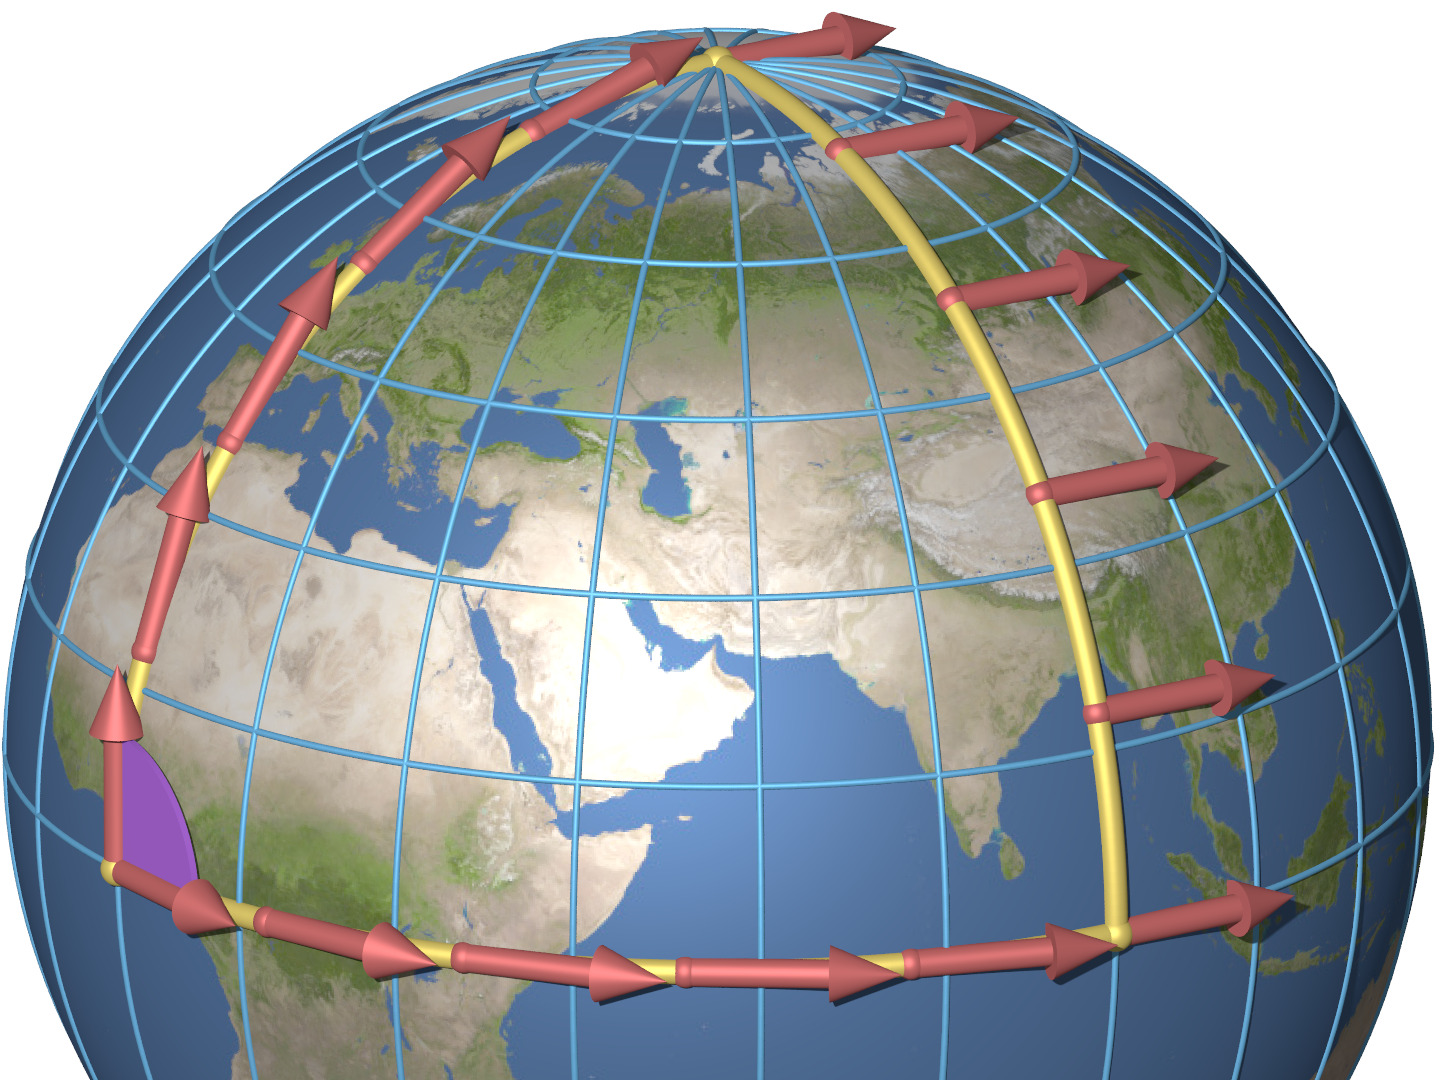
\includegraphics[width=9cm]{chapters/000-einleitung/images/kruemmung.jpg}
\caption{Der Paralleltransport des roten Vektors zunächst entlang des
Äquators, dann entlang eines Längenkreises zum Nordpol und schliesslich
entlang eines weiteren Längenkreises zurück zum Ausgangspunkt führt zu
einer von der Krümmung der Kugeloberfläche verursachten Drehung des
Vektors um den violetten $90^\circ$-Winkel.
\label{buch:einleitung:fig:kruemmung}}
\end{figure}
